\chapter{Aging riveted bridge}
\label{app2}
\onehalfspacing


\subsection{Microscope observation}\label{app-obsur}

As shown in Fig. \ref{ch3fig3}, the joint surface was observed with an electron microscope of 60, 200 and 600 times. The orange-red substance is red lead (Pb3O4), and the black primer is the black oxide of steel (Fe2O3). No obvious traces of rust are found on the joint surface. The light reflecting material in the picture is a resin coating.

\begin{figure}
    \centering
    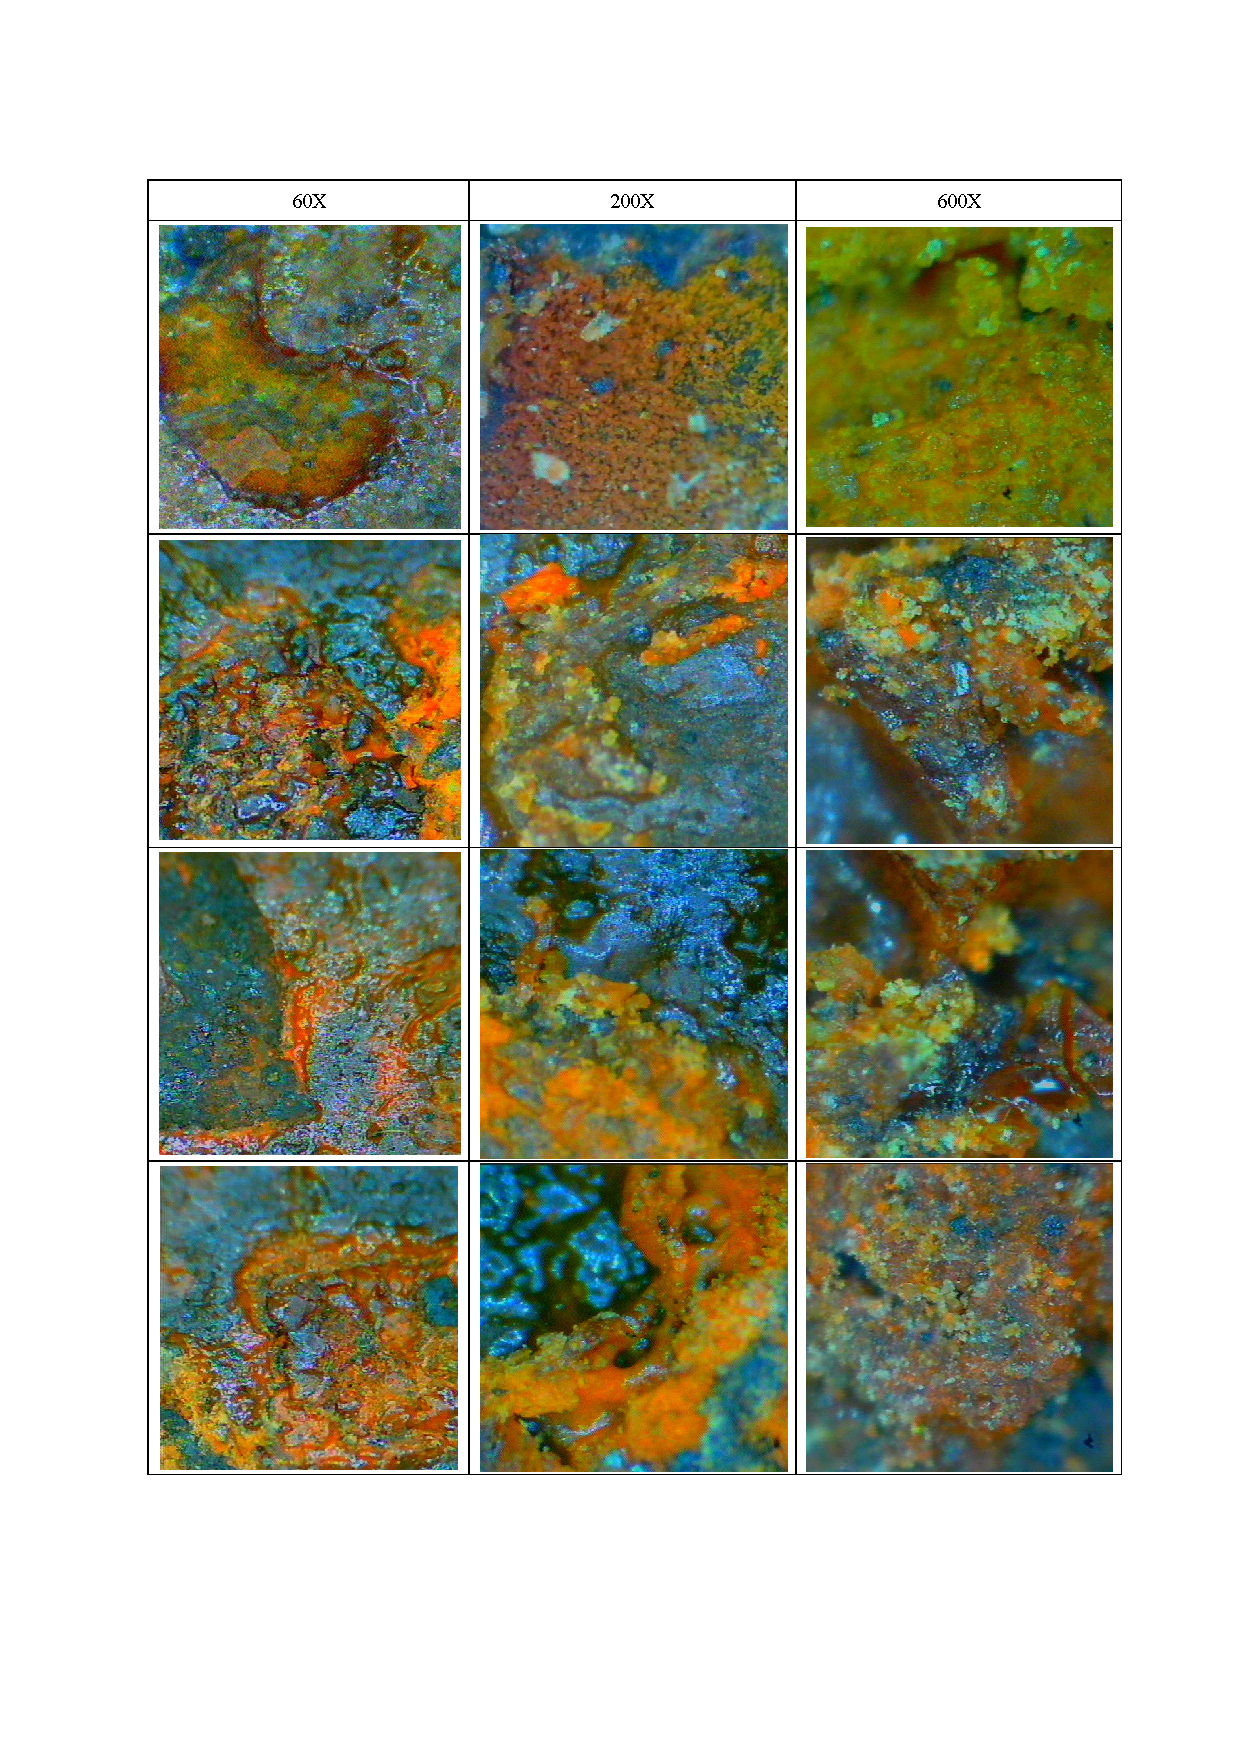
\includegraphics[width=1\linewidth]{imgs//app2/fig-ob-surface.pdf}
    \caption{Microscope observation for faying surface of riveted joint}
    \label{fig-obsur}
\end{figure}


\section{Lamination of riveted joint main plate}

Laminations are an imperfection in a steel, resulting from blisters, seams, foreign material, and/or scratches on an ingot or billet that are not repaired during the rolling process.

Due to the immaturity of previous steelmaking technology, impurities or air bubbles were present in the steelmaking process, leading to the appearance of lamination, which resulted in unexpected damage to the material during testing and lower than expected strength values as shown in Fig. \ref{fig-lami}.

In this experiment, multiple laminations were found only in the web of one riveted girder, which is particularly important for evaluating the load carrying capacity of riveted bridges.

\begin{figure}
    \centering
    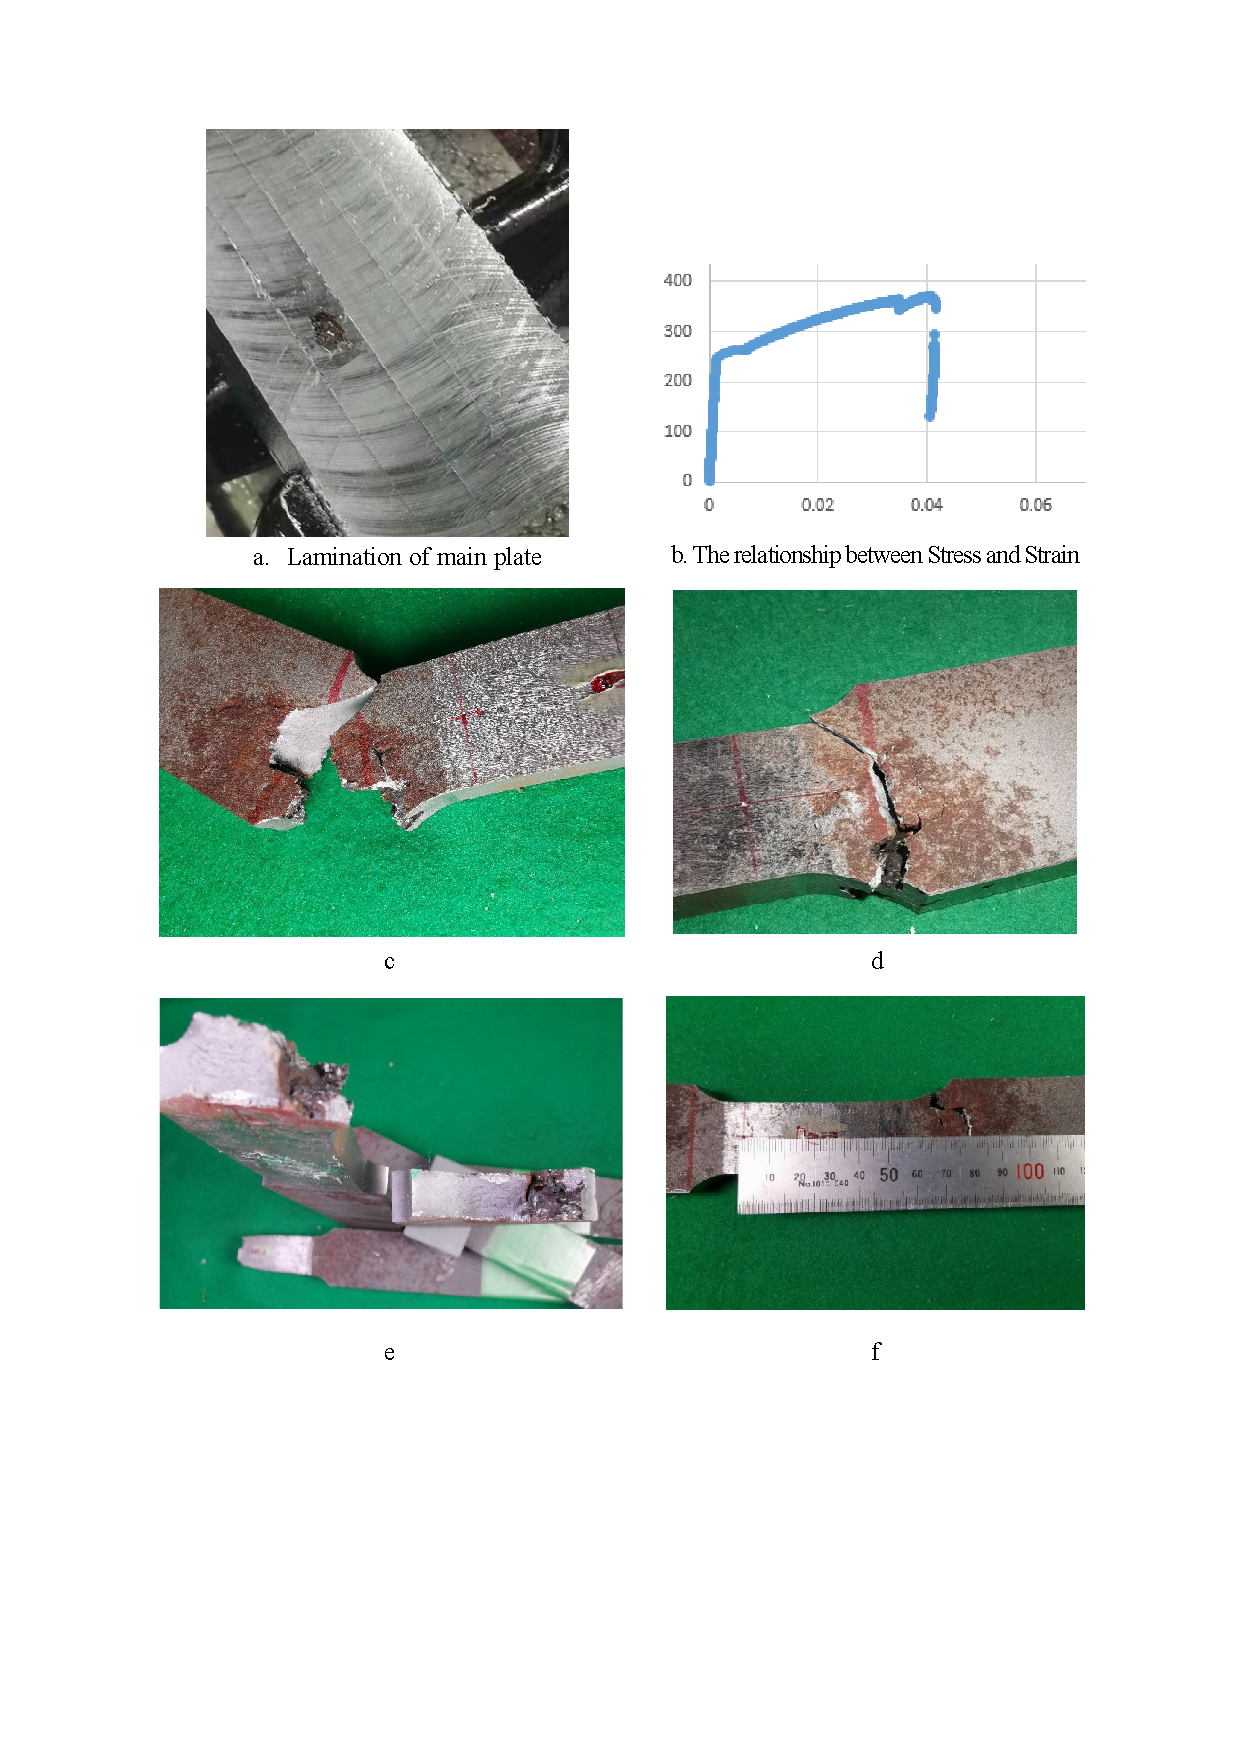
\includegraphics[width=1\linewidth]{imgs//app2/fig-lami.pdf}
    \caption{Lamination of main plate}
    \label{fig-lami}
\end{figure}